\chapter{Benchmark Specification}
\label{section:benchmark-specification}

\section{Requirements}

\ldbcsnb is designed to be flexible and to have an affordable entry point.
From small single node and in memory systems to large distributed multi-node
clusters have its own place in \ldbcsnb.  Therefore, the requirements to
fulfill for executing \ldbcsnb are limited to pure software requirements to be
able to run the tools. All the software provided by \ldbcsnb have been
developed and tested under Linux-based operating systems.

\ldbcsnb does not impose the usage of any specific type of system, as it
targets systems of different nature and characteristics, from graph databases,
graph processing frameworks and RDF systems, to traditional relational database
management systems. Consequently, any language or API capable of expressing the
proposed queries can be used. Similarly, data can be stored in the most
convenient manner the test sponsor may decide.

%, as long as it conforms with the
%execution rules. Finally, in order to have an official benchmark execution, the
%results will have to be audited and all the required information disclosed.

%%%%%%%%%%%%%%%%%%%%%%%%%%%%%%%%%%%%%%%%%%%%%%%%%%%%%%%%%%%%%%%%%%%%%%%%%%%%%%
%%%%%%%%%%%%%%%%%%%%%%%%%%%%%%%%%%%%%%%%%%%%%%%%%%%%%%%%%%%%%%%%%%%%%%%%%%%%%%
%%%%%%%%%%%%%%%%%%%%%%%%%%%%%%%%%%%%%%%%%%%%%%%%%%%%%%%%%%%%%%%%%%%%%%%%%%%%%%

\section{Software and Useful Links}

\begin{itemize}
    \item \textbf{LDBC Driver -- \url{https://github.com/ldbc/ldbc_driver}}: The driver
    responsible for executing the \ldbcsnb workload.
    \item \textbf{\datagen{} -- \url{https://github.com/ldbc/ldbc_snb_datagen}}: The data
    generator used to generate the datasets of the benchmark.
\end{itemize}

%%%%%%%%%%%%%%%%%%%%%%%%%%%%%%%%%%%%%%%%%%%%%%%%%%%%%%%%%%%%%%%%%%%%%%%%%%%%%%
%%%%%%%%%%%%%%%%%%%%%%%%%%%%%%%%%%%%%%%%%%%%%%%%%%%%%%%%%%%%%%%%%%%%%%%%%%%%%%
%%%%%%%%%%%%%%%%%%%%%%%%%%%%%%%%%%%%%%%%%%%%%%%%%%%%%%%%%%%%%%%%%%%%%%%%%%%%%%

\section{Data}
\label{section:data}

This section introduces the data used by \ldbcsnb. This includes the different
data types, the data schema, how it is generated and the different scale
factors.

\subsection{Data Types}
\autoref{table:types} describes the different data types used in the benchmark.

\begin{table}[h]
\centering
\begin{tabular}{|>{\typeCell}p{\attributeColumnWidth}|p{\largeDescriptionColumnWidth}|}
    \hline
    \tableHeaderFirst{Type} & \tableHeader{Description} \\
    \hline
    ID &  integer type with 64-bit precision. All IDs within a single entity type (\eg Post) are unique, but different entity types (\eg a Forum and a Post) might have the same ID.\\
    \hline
    32-bit Integer &  integer type with 32-bit precision\\
    \hline
    64-bit Integer &  integer type with 64-bit precision\\
    \hline
    String & variable length text of size 40 Unicode characters\\
    \hline
    Long String & variable length text of size 256 Unicode characters\\
    \hline
    Text &  variable length text of size 2000 Unicode characters\\
    \hline
    Date &  date with a precision of a day, encoded as a string with the following format: \textit{yyyy-mm-dd}, where \textit{yyyy} is a four-digit integer representing the year,
    the year, \textit{mm} is a two-digit integer representing the month and \textit{dd} is a two-digit integer representing the day. \\
    \hline
    DateTime &  date with a precision of milliseconds, encoded as a string with the following format: \textit{yyyy-mm-ddTHH:MM:ss.sss+0000}, where \textit{yyyy} is a four-digit integer representing the year,
    the year, \textit{mm} is a two-digit integer representing the month and \textit{dd} is a two-digit integer representing the day, \textit{HH} is a two-digit integer representing the hour, \textit{MM} is a two
    digit integer representing the minute and \textit{ss.sss} is a five digit fixed point real number representing the seconds up to millisecond precision. Finally, the \textit{+0000} of the end represents the
    timezone, which in this case is always GMT.\\
    \hline
    Boolean &  logical type, taking the value of either True of False\\
    \hline
\end{tabular}
\caption{Description of the data types.}
\label{table:types}
\end{table}


\subsection{Data Schema}

\autoref{figure:schema} shows the data schema in UML. The schema defines the
structure of the data used in the benchmark in terms of entities and their
relations. Data represents a snapshot of the activity of a social network
during a period of time. Data includes entities such as Persons, Organisations,
and Places. The schema also models the way persons interact, by means of the
friendship relations established with other persons, and the sharing of content
such as messages (both textual and images), replies to messages and likes to
messages.  People form groups to talk about specific topics, which are
represented as tags.

\ldbcsnb has been designed to be flexible and to target systems of different
nature and characteristics. As such, it does not force any particular internal
representation of the schema. The \datagen component
% described in \autoref{section:data_generation}
supports multiple output data formats to
fit the needs of different types of systems, including RDF, relational DBMS and
graph DBMS.

\begin{figure}[htbp]
    \centering
    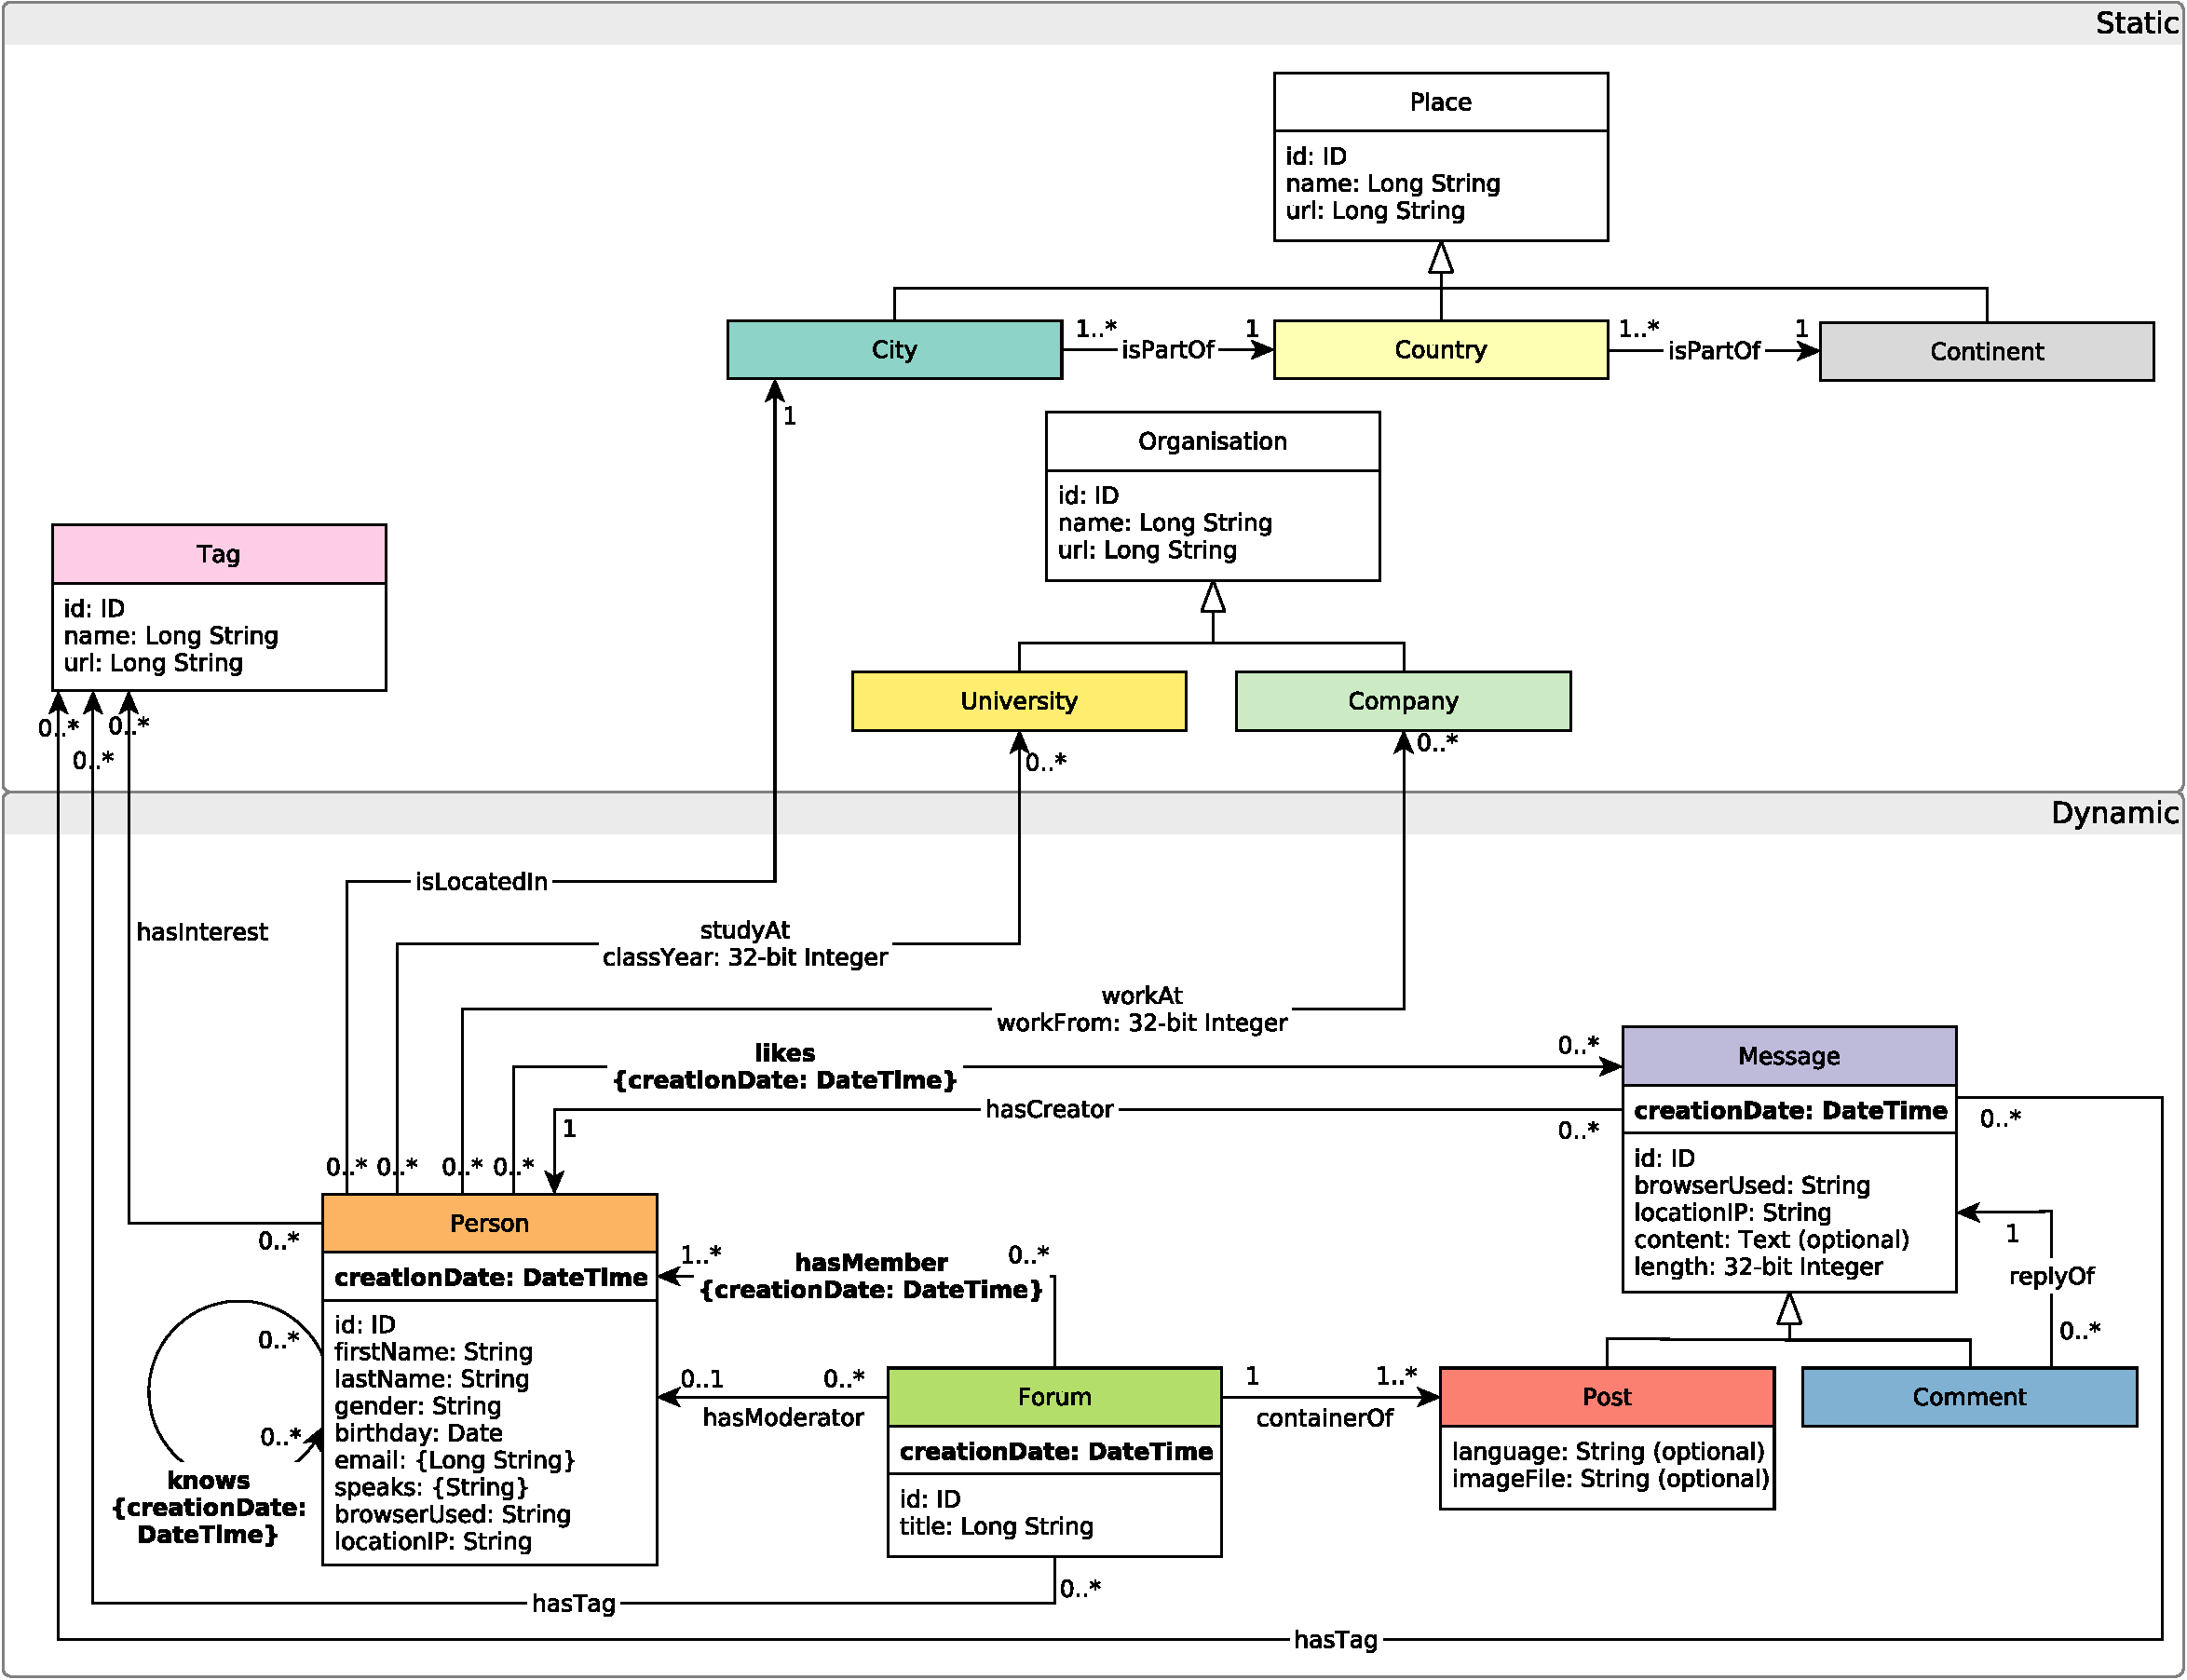
\includegraphics[width=\linewidth]{figures/schema-comfortable}
    \caption{UML class diagram-style depiction of the \ldbcsnb graph schema. Note that the \textsf{knows} edges are represented as directed but should be treated as undirected.}
    \label{figure:schema}
\end{figure}

The schema specifies different entities, their attributes and their relations.
All of them are described in the following sections.

{\flushleft \textbf{Textual Restrictions and Notes}}
\begin{itemize}
    \item Posts have content or imageFile. They have one of them but not both. The one they do not have is an empty string.\footnote{Implementations can use other means to represent this value such as a \texttt{NULL}.}
    \item Posts in a forum can be created by a non-member person if and only if that person is a moderator.
\end{itemize}

\subsubsection{Entities}

{\flushleft \textbf{City:}} a sub-class of a Place, and represents a
city of the real world. City entities are used to specify where persons live,
as well as where universities operate.

{\flushleft \textbf{Comment:}} a sub-class of a Message, and represents a
comment made by a person to an existing message (either a Post or a Comment).

{\flushleft \textbf{Company:}} a sub-class of an Organisation, and represents a company where persons work.


{\flushleft \textbf{Country:}} a sub-class of a Place, and represents a continent of the real world.


{\flushleft \textbf{Forum:}} a meeting point where people
post messages. Forums are characterized by the topics (represented as tags)
people in the forum are talking about. Although from the schema's perspective
it is not evident, there exist three different types of
forums.  They are distinguished by their titles:

\begin{itemize}
    \item persons' personal walls: ``Wall of \ldots''
    \item image albums: ``Album $k$ of \ldots''
    \item groups: ``Group for \ldots''
\end{itemize}

\autoref{table:forum} shows the attributes of Forum entity.

\begin{table}[H]
    \begin{tabular}{|>{\varNameCell}p{\attributeColumnWidth}|>{\typeCell}p{\typeColumnWidth}|p{\descriptionColumnWidth}|}
        \hline
        \tableHeaderFirst{Attribute} & \tableHeader{Type} & \tableHeader{Description} \\
        \hline
        id & ID  & The identifier of the forum.\\
        \hline
        title & Long String  & The title of the forum.\\
        \hline
        creationDate & DateTime  & The date the forum was created.\\
        \hline
    \end{tabular}
    \caption{Attributes of Forum entity.}
    \label{table:forum}
\end{table}

{\flushleft \textbf{Message:}} an abstract entity that represents a message
created by a person. \autoref{table:message} shows the attributes of Message
abstract entity.

\begin{table}[H]
    \begin{tabular}{|>{\varNameCell}p{\attributeColumnWidth}|>{\typeCell}p{\typeColumnWidth}|p{\descriptionColumnWidth}|}
        \hline
        \tableHeaderFirst{Attribute} & \tableHeader{Type} & \tableHeader{Description} \\
        \hline
        id & ID  & The identifier of the message.\\
        \hline
        browserUsed & String  & The browser used by the Person to create the message.\\
        \hline
        creationDate & DateTime  & The date the message was created.\\
        \hline
        locationIP & String  & The IP of the location from which the message was created.\\
        \hline
        content & Text[0..1]  & The content of the message.\\
        \hline
        length & 32-bit Integer  & The length of the content.\\
        \hline
    \end{tabular}
    \caption{Attributes of Message interface.}
    \label{table:message}
\end{table}

{\flushleft \textbf{Organisation:}} an institution of the real
world. \autoref{table:organisation} shows the attributes of Organisation
entity.

\begin{table}[H]
    \begin{tabular}{|>{\varNameCell}p{\attributeColumnWidth}|>{\typeCell}p{\typeColumnWidth}|p{\descriptionColumnWidth}|}
        \hline
        \tableHeaderFirst{Attribute} & \tableHeader{Type} & \tableHeader{Description} \\
        \hline
        id & ID  & The identifier of the organisation.\\
        \hline
        name & Long String  & The name of the organisation.\\
        \hline
        url & Long String  & The URL of the organisation.\\
        \hline
    \end{tabular}
    \caption{Attributes of Organisation entity.}
    \label{table:organisation}
\end{table}

{\flushleft \textbf{Person:}} the avatar a real world person creates
when he/she joins the network, and contains various information about the
person as well as network related information. \autoref{table:person} shows
the attributes of Person entity.

\begin{table}[H]
    \begin{tabular}{|>{\varNameCell}p{\attributeColumnWidth}|>{\typeCell}p{\typeColumnWidth}|p{\descriptionColumnWidth}|}
        \hline
        \tableHeaderFirst{Attribute} & \tableHeader{Type} & \tableHeader{Description} \\
        \hline
        id & ID  & The identifier of the person.\\
        \hline
        firstName & String  & The first name of the person.\\
        \hline
        lastName & String  & The last name of the person.\\
        \hline
        gender & String  & The gender of the person.\\
        \hline
        birthday & Date  & The birthday of the person.\\
        \hline
        email & Long String[1..*]  & The set of emails the person has.\\
        \hline
        speaks & String[1..*]  & The set of languages the person speaks.\\
        \hline
        browserUsed & String  & The browser used by the person when he/she registered to the social network.\\
        \hline
        locationIP & String  & The IP of the location from which the person was registered to the social network.\\
        \hline
        creationDate & DateTime  & The date the person joined the social network.\\
        \hline
    \end{tabular}
    \caption{Attributes of Person entity.}
    \label{table:person}
\end{table}


{\flushleft \textbf{Place:}} a place in the world.
\autoref{table:place} shows the attributes of Place entity. Note, each Place has additional parameters: longitude and latitude, which are not exposed. These are used internally for sorting places.

\begin{table}[H]
    \begin{tabular}{|>{\varNameCell}p{\attributeColumnWidth}|>{\typeCell}p{\typeColumnWidth}|p{\descriptionColumnWidth}|}
        \hline
        \tableHeaderFirst{Attribute} & \tableHeader{Type} & \tableHeader{Description} \\
        \hline
        id & ID  & The identifier of the place.\\
        \hline
        name & Long String  & The name of the place.\\
        \hline
        url & Long String  & The URL of the place.\\
        \hline
    \end{tabular}
    \caption{Attributes of Place entity.}
    \label{table:place}
\end{table}

{\flushleft \textbf{Post:}} a sub-class of Message, that is posted in a
forum. Posts are created by persons into the forums where they belong.
Posts contain either content or imageFile, always one of them but never both.
The one they do not have is an empty string.
\autoref{table:post} shows the attributes of Post entity.

\begin{table}[H]
    \begin{tabular}{|>{\varNameCell}p{\attributeColumnWidth}|>{\typeCell}p{\typeColumnWidth}|p{\descriptionColumnWidth}|}
        \hline
        \tableHeaderFirst{Attribute} & \tableHeader{Type} & \tableHeader{Description} \\
        \hline
        language & String[0..1]  & The language of the post.\\
        \hline
        imageFile & String[0..1]  & The image file of the post.\\
        \hline
    \end{tabular}
    \caption{Attributes of Post entity.}
    \label{table:post}
\end{table}

{\flushleft \textbf{Tag:}} a topic or a concept. Tags are used to
specify the topics of forums and posts, as well as the topics a person is
interested in. \autoref{table:tag} shows the attributes of Tag entity.

\begin{table}[H]
    \begin{tabular}{|>{\varNameCell}p{\attributeColumnWidth}|>{\typeCell}p{\typeColumnWidth}|p{\descriptionColumnWidth}|}
        \hline
        \tableHeaderFirst{Attribute} & \tableHeader{Type} & \tableHeader{Description} \\
        \hline
        id & ID  & The identifier of the tag.\\
        \hline
        name & Long String  &  The name of the tag.\\
        \hline
        url & Long String  &  The URL of the tag.\\
        \hline
    \end{tabular}
    \caption{Attributes of Tag entity.}
    \label{table:tag}
\end{table}

{\flushleft \textbf{TagClass:}} a class used to build a hierarchy of tags. \autoref{table:tagclass} shows the attributes of TagClass entity.

\begin{table}[H]
    \begin{tabular}{|>{\varNameCell}p{\attributeColumnWidth}|>{\typeCell}p{\typeColumnWidth}|p{\descriptionColumnWidth}|}
        \hline
        \tableHeaderFirst{Attribute} & \tableHeader{Type} & \tableHeader{Description} \\
        \hline
        id & ID  & The identifier of the tagclass.\\
        \hline
        name & Long String  &  The name of the tagclass.\\
        \hline
        url & Long String  &  The URL of the tagclass.\\
        \hline
    \end{tabular}
    \caption{Attributes of TagClass entity.}
    \label{table:tagclass}
\end{table}

{\flushleft \textbf{University:}} a sub-class of Organisation,
and represents an institution where persons study.

\subsubsection{Relations}

Relations connect entities of different types. Entities are defined by their ''id'' attribute.

\begin{longtable}{|>{\varNameCell}p{2.5cm}|>{\typeCell}p{2.5cm}|>{\typeCell}p{2.5cm}|>{\edgeDirectionCell}c|p{6.5cm}|}
       \hline
        \tableHeaderFirst{Name} & \tableHeader{Tail} & \tableHeader{Head} & \tableHeader{Type} & \tableHeader{Description} \\
        \hline
        containerOf & Forum[1] & Post[1..*] & D & A Forum and a Post contained in it\\
        \hline
        hasCreator & Message[0..*] & Person[1] & D & A Message and its creator (Person)\\
        \hline
        hasInterest & Person[0..*] & Tag[0..*] & D & A Person and a Tag representing a topic the person is interested in\\
        \hline
        hasMember & Forum[0..*] &  Person[1..*] & D & A  Forum and a member (Person) of the forum

        \attributeTable{creationDate}{DateTime}{The Date the person joined the forum}

        \\
        \hline
        hasModerator & Forum[0..*] & Person[1] & D & A Forum and its moderator (Person) \\
        \hline
        hasTag & Message[0..*] & Tag[0..*] & D & A Message and a Tag representing the message's topic \\
        \hline
        hasTag & Forum[0..*] & Tag[0..*] & D & A Forum and a Tag representing the forum's topic \\
        \hline
        hasType & Tag[0..*] & TagClass[1] & D & A Tag and a TagClass the tag belongs to \\
        \hline
        isLocatedIn & Company[0..*] & Country[1] & D & A Company and its home Country \\
        \hline
        isLocatedIn & Message[0..*] & Country[1] & D & A Message and the Country from which it was issued \\
        \hline
        isLocatedIn & Person[0..*] & City[1] & D & A Person and their home City \\
        \hline
        isLocatedIn & University[0..*] & City[1] & D &  A University and the City where the university is \\
        \hline
        isPartOf & City[1..*] & Country[1] & D & A City and the Country it is part of \\
        \hline
        isPartOf & Country[1..*] & Continent[1] & D & A Country and the Continent it is part of \\
        \hline
        isSubclassOf & TagClass[0..*] & TagClass[0..1] & D & A TagClass and its parent TagClass \\
        \hline
        knows & Person[0..*] & Person[0..*] & U & Two Persons that know each other

        \attributeTable{creationDate}{DateTime}{The date the knows relation was established}

        \\
        \hline
        likes & Person[0..*] & Message[0..*] & D & A Person that likes a Message

        \attributeTable{creationDate}{DateTime}{The date the like was issued}

        \\
        \hline
        replyOf & Comment[0..*] & Message[1] & D & A Comment and the Message it replies \\
        \hline
        studyAt & Person[0..*] & University[0..*] & D & A Person and a University it has studied

        \attributeTable{classYear}{32-bit Integer}{The year the person graduated}

        \\
        \hline
        workAt & Person[0..*] & Company[0..*] & D & A Person and a Company it works

        \attributeTable{workFrom}{32-bit Integer}{The year the person started to work at that company}

        \\
        \hline
    \caption{Description of the data relations. \texttt{D}: directed edge, \texttt{U}: undirected edge.}
        \label{table:relations}
\end{longtable}

\subsubsection{Domain Concepts}

A \emph{thread} consists of Messages, starting with a single Post and Comments that transitively reply to that Post.

\subsection{Data Generation}
\label{section:data_generation}

\ldbcsnb provides \datagen (Data Generator), which produces synthetic
datasets following the schema described above. Data
produced mimics a social network's activity during a period of time. Three
parameters determine the generated data: the number of persons, the number of
years simulated, and the starting year of simulation. \datagen is defined by the
following characteristics:

\begin{itemize}
    \item \textbf{Realism.} Data generated by \datagen mimics the
        characteristics of those found in a real social network. In \datagen,
        output attributes, cardinalities, correlations and distributions have
        been finely tuned to reproduce a real social network in each of its
        aspects On the one hand, it is aware of the  data and link distributions
        found in a real social network such as Facebook. On the other hand, it
        uses real data from DBpedia, such as property dictionaries, which are
        used to ensure that attribute values are realistic and correlated.
    \item \textbf{Scalability.} Since \ldbcsnb targets systems of different
        scales and budgets, \datagen is capable of generating datasets of
        different sizes, from a few Gigabytes to Terabytes. \datagen is
        implemented following the MapReduce parallel paradigm, allowing the
        generation of small datasets in single node machines, as well as large
        datasets on commodity clusters.
    \item \textbf{Determinism.} \datagen is deterministic regardless of the number
        of cores/machines used to produce the data. This important feature
        guarantees that all Test Sponsors will face the same dataset,
        thus, making the comparisons between different systems fair and the
        benchmarks' results reproducible.
    \item \textbf{Usability.} \ldbcsnb is designed to have an affordable entry
        point. As such, \datagen's design is  severely influenced by this
        philosophy, and therefore it is designed to be as easy to use as
        possible.
\end{itemize}


\subsubsection{Resource Files}

\datagen uses a set of resource files with data
extracted from DBpedia. Conceptually, \datagen generates attribute's
values following a property dictionary model that is defined by

\begin{itemize}
    \item a dictionary $D$
    \item a ranking function $R$
    \item a probability function $F$
\end{itemize}

Dictionary D is a fixed set of values. The ranking function R is a bijection
that assigns to each value in a dictionary a unique rank between 1 and |$D$|.
The probability density function $F$ specifies how the data generator chooses
values from dictionary $D$ using the rank for each term in the dictionary. The
idea to have a separate ranking and probability function is motivated by the
need of generating correlated values: in particular, the ranking function is
typically parameterized by some parameters: different parameter values result
in different rankings. For example, in the case of a dictionary of property
firstName, the popularity of first names, might depend on the gender, country
and birthday properties. Thus, the fact that the popularity of first names in
different countries and times is different, is reflected by the different ranks
produced by function $R$ over the full dictionary of names.  \datagen uses a
dictionary for each literal property, as well as ranking functions for all
literal properties. These are materialized in a set of resource files, which
are described in \autoref{table:property_dictionaries}.

\begin{table}[H]
\begin{tabular}{|p{4cm}|p{12cm}|}
    \hline
    \tableHeaderFirst{Resource Name} & \tableHeader{Description} \\
    \hline
    Browsers & Contains a list of web browsers and their probability to be used. It is used to set the browsers used by the users.\\
    \hline
    Cities by Country & Contains a list of cites and the country they belong. It is used to assign cities to users and universities.\\
    \hline
    Companies by Country & Contains the set of companies per country. It is used to set the countries where companies operate.\\
    \hline
    Countries & Contains a list of countries and their populations. It is used to obtain the amount of people generated for each country.\\
    \hline
    Emails & Contains the set of email providers. It is used to generate the email accounts of persons.\\
    \hline
    IP Zones & Contains the set of IP ranges assigned to each country. It is used to assign the IP addresses to users.\\
    \hline
    Languages by Country & Contains the set of languages spoken in each country. It is used to set the languages spoken by each user.\\
    \hline
    Name by Country & Contains the set of names and the probability to appear in each country. It is used to assign names to persons, correlated with their countries.\\
    \hline
    Popular places by Country & Contains the set of popular places per country. These are used to set where images attached to posts are taken from.\\
    \hline
    Surnames' by Country & Contains the set of surnames and the probability to appear in each country. It is used to assign surnames to persons, correlated with their countries.\\
    \hline
    Tags by Country & Contains a set of tags and their probability to appear in each country. It is used to assign the interests to persons and forums.\\
    \hline
    Tag Classes & Contains, for each tag, the classes it belongs to.\\
    \hline
    Tag Hierarchies & Contains, for each tagClass, their parent tagClass.\\
    \hline
    Tag Matrix & Contains, for each tag, the correlation probability with the other tags. It is used enrich the tags associated to messages.\\
    \hline
    Tag Text & Contains, for each tag, a text. This is used to generate the text for messages.\\
    \hline
    Universities by City & Contains the set of universities per city. It is used to set the cities where universities operate.\\
    \hline
\end{tabular}
    \caption{Resource files}
    \label{table:property_dictionaries}
\end{table}

\subsubsection{Graph Generation}



% also used to generate lcoation

\autoref{figure:generation_process} conceptually depicts the full data
generation process. The first step loads all the dictionaries and resource
files, and initializes the \datagen parameters.  Second, it generates all the
Persons in the graph, and the minimum necessary information to operate. Part of
these information are the interests of the persons, and the number of knows
relationships of every person, which is guided by a degree distribution
function similar to that found in Facebook~\cite{facebook_anatomy}.

The next three steps are devoted to the creation of knows relationships.  An
important aspect of real social networks, is the fact that similar persons
(with similar interests and behaviors) tend to be connected. This is known as
the Homophily principle~\cite{mcpherson2001birds,DBLP:journals/socnet/BaroneC18}, and implies the presence of
a larger amount of triangles than that expected in a random network. In order
to reproduce this characteristic, \datagen generates the edges by means of
correlation dimensions.  Given a person, the probability to be connected to
another person is typically skewed with respect to some similarity between the
persons. That is, for a person $p$ and for a small set of persons that are
somehow similar to it, there is a high connectivity probability, whereas for
most other persons, this probability is quite low. This knowledge is
exploited by \datagen to reproduce correlations.

\begin{figure}[H]
    \centering
    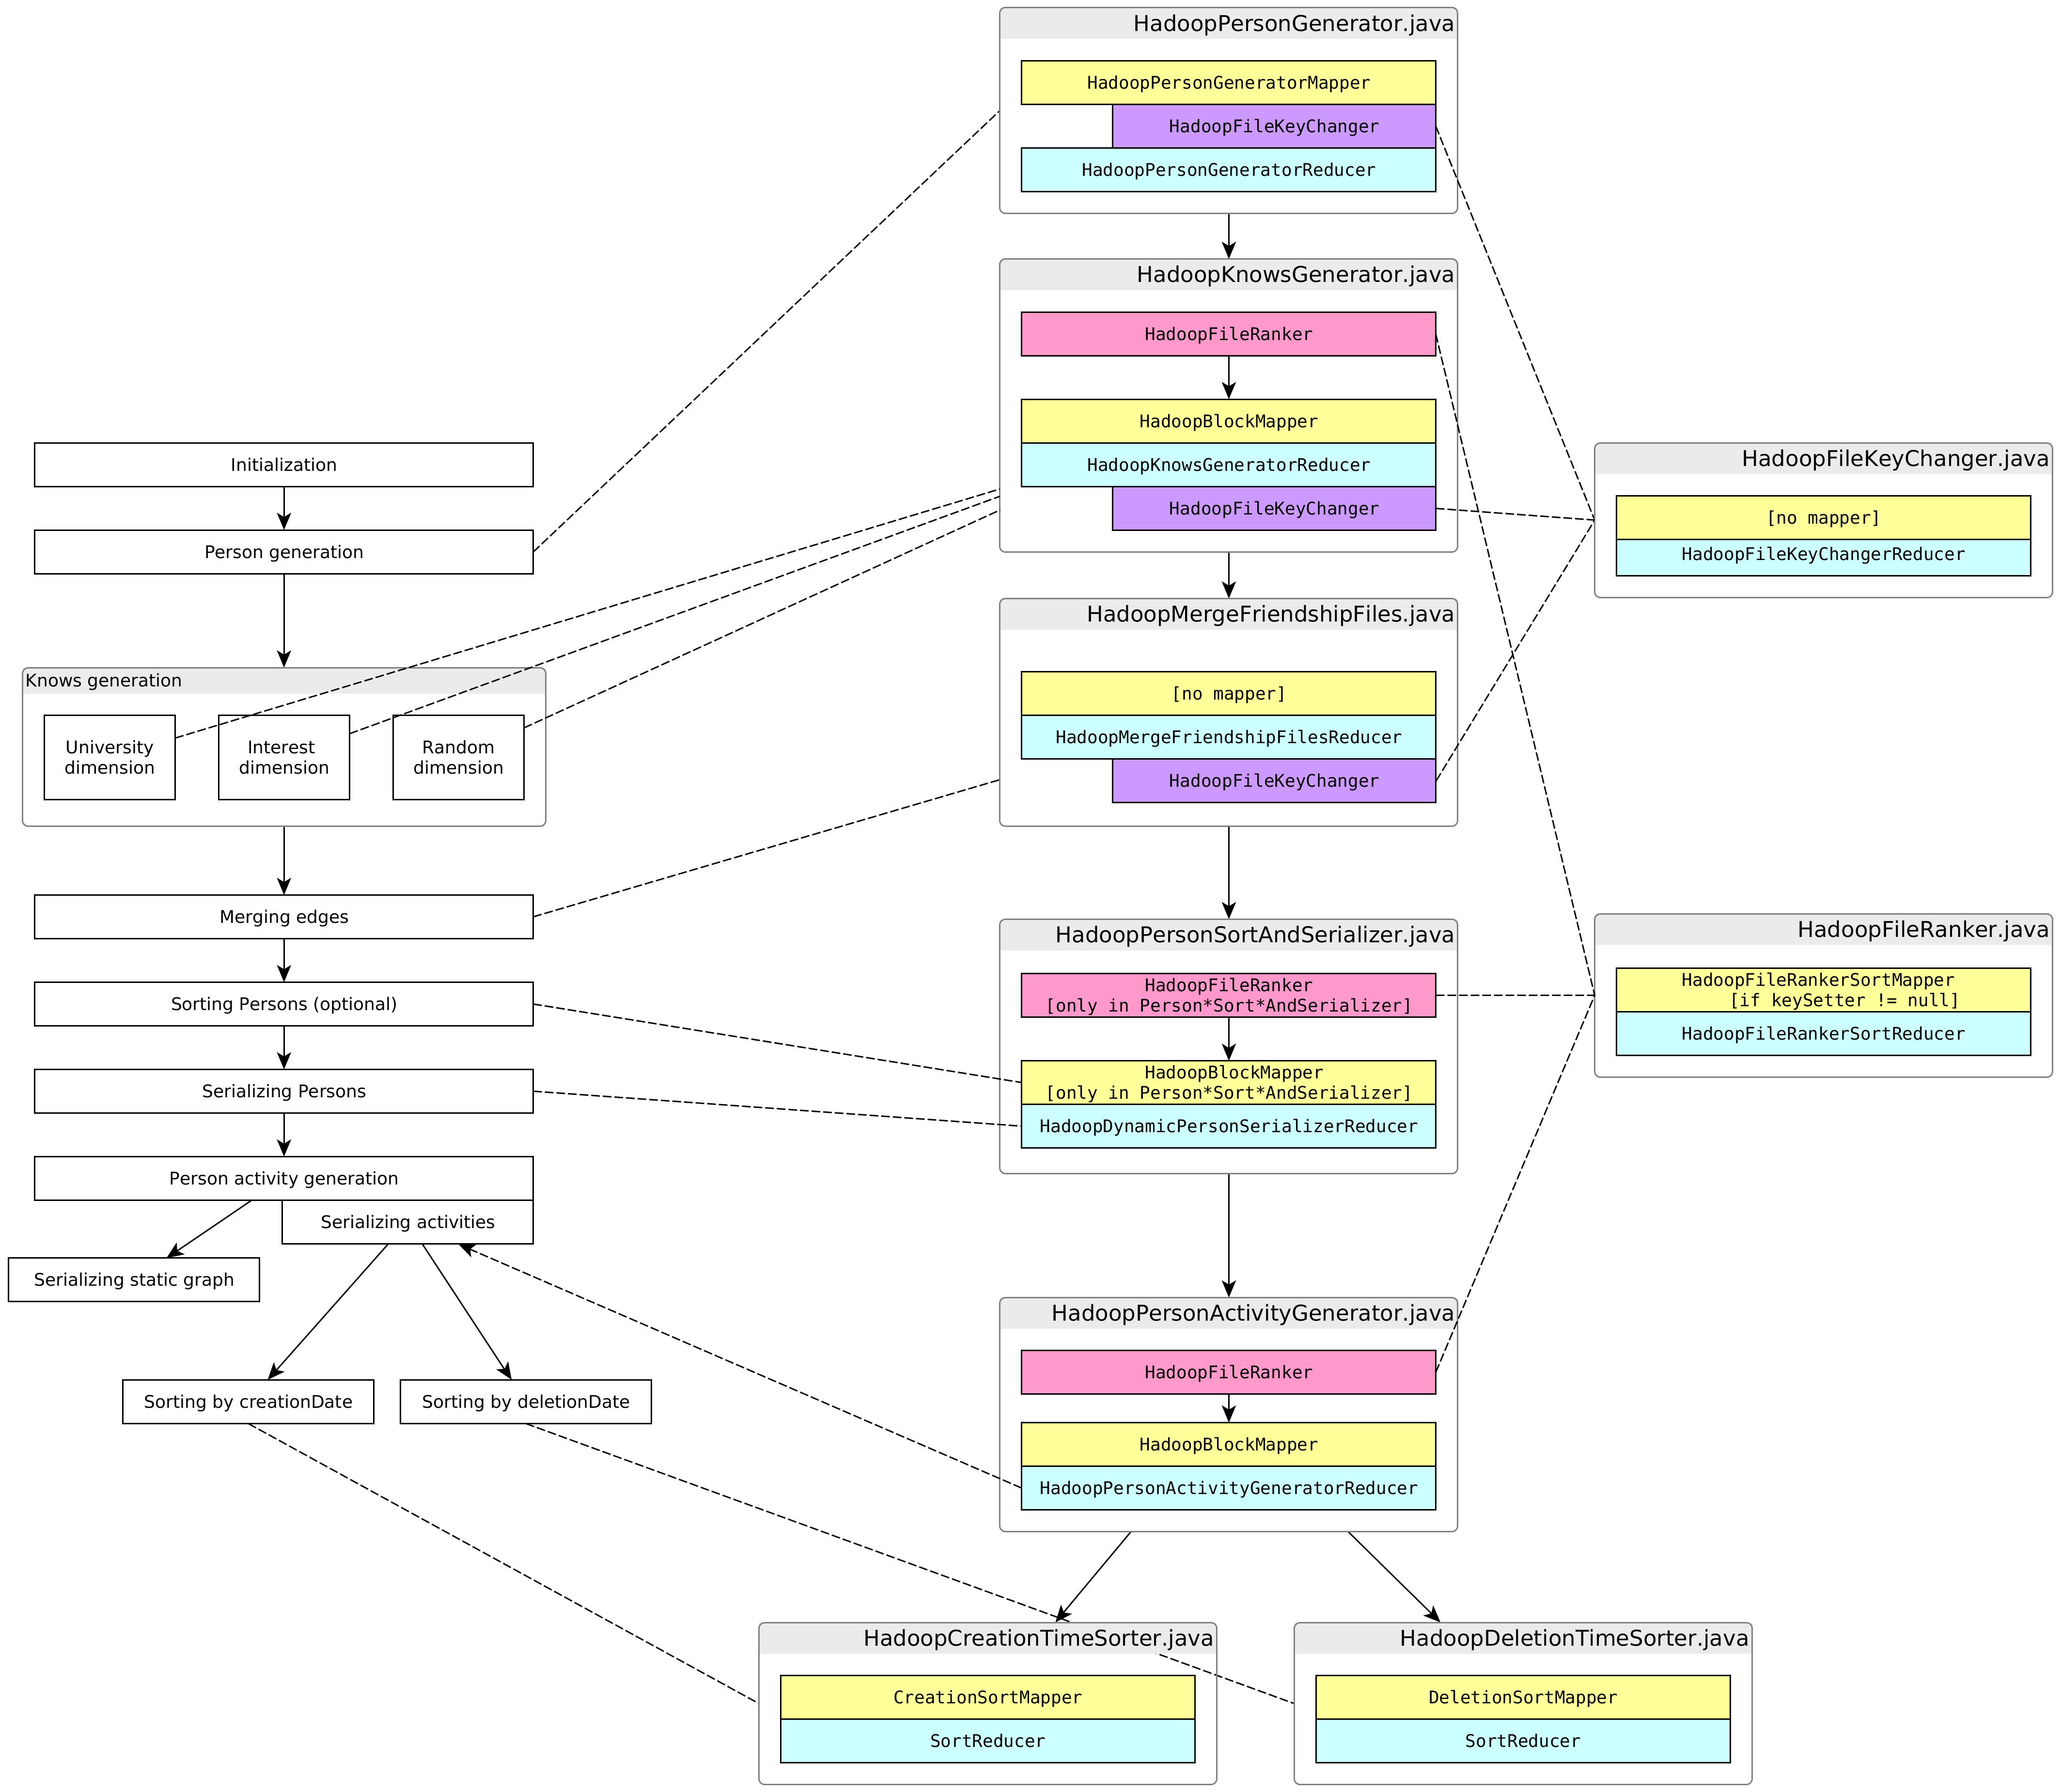
\includegraphics[scale=\patternscale]{figures/datagen-workflow}
    \caption{The \datagen generation process.}
    \label{figure:generation_process}
\end{figure}

Given a similarity function $M(p) : p \rightarrow [0, \infty]$ that gives a score to a person,
with the characteristic that two similar persons will have similar scores, we
can sort all the persons by function $M$ and compare a person $p$ against only the
$K$ neighboring persons in the sorted array. The consequence of this approach is
that similar persons are grouped together, and the larger the
distance between two persons indicates a monotonic increase in their similarity
difference. In order to choose the persons to connect, \datagen uses a geometric
probability distribution that provides a probability for picking persons to
connect, that are between 1 and $K$ positions apart in the similarity
ranking.

Similarity functions and probability distribution functions over ranked
distance drive what kind of persons will be connected with an edge, not how
many. As stated above, the number of friends of a person is determined by a
Facebook-like distribution. The edges that will be connected to a person $p$,
are selected by randomly picking the required number of edges according to the
correlated probability distributions as discussed before. In the case that
multiple correlations exist, another probability function is used to divide the
intended number of edges between the various correlation dimensions. In \datagen,
three correlated dimensions are chosen: the first one depends on where the
person studied and when, and the second correlation dimension depends on the
interests of the person, and the third one is random (to reproduce the random
noise present in real data). Thus, \datagen has a Facebook-like distributed node
degree, and a predictable (but not fixed) average split between the reasons for
creating edges.

In the next step, person's activity, in the form of forums, posts and comments
is created. \datagen reproduces the fact that people with a larger number of
friends have a higher activity, and hence post more photos and comments to a
larger number of posts. Another important characteristic of real users'
activity in social network, are time correlations.  Usually, users' posts
creation in a social network is driven by real world events.  For
instance, one may think about an important event such as the elections in a
country, or a natural disaster. Around the time these events occur, network
activity about these events' topics sees an increase in volume. \datagen
reproduces these characteristics with the simulation of what we name as
flashmob events.  Several events are generated randomly at the beginning of the
generation process, which are assigned a random tag, and are given a time and
an intensity which represents the repercussion of the event in the real world.
When persons' posts are created, some of them are classified as flashmob posts,
and their topics and dates are assigned based on the generated flashmob events.
The volume of activity around this events is modeled following a model similar
to that described in~\cite{DBLP:conf/kdd/LeskovecBKT08}. Furthermore, in order to reproduce the
more uniform every day's user activity, \datagen also generates post uniformly
distributed along all the simulated time.

Finally, in the last step the data is serialized into the output files.

\subsubsection{Distributions, Parameters and Quirks}
\label{sec:distr-param}

Interesting quirks:
\begin{itemize}
\item A Person is not a member of their Wall but they are its moderator, they do not have a hasMember edge.
\item Each Album generated for Person will have approximately 70\% of their friends as members.
\item A given Person has a 5\% chance of being a moderator of a set of groups.
\item Group membership is composed of 30\% from the moderator's friends and the remainder is chosen randomly (from the block the person is in).
\item Comments are only made in Walls and Groups.
\item Messages can only receive likes during a 7-day window after their creation.
\item Comments always occur within one day of Message they are replying to. The creation date is generated following the power-law distribution in Figure \ref{figure:comments_dist}. The mean lag between Comments and their parent Message is 6.85 hours.
\item Flashmob events span a 72 hour time window with a specific event time in the middle of the window; there are 36 hours each side of the specific event time. Following the distribution in Figure \ref{figure:flashmob_dist} posts are generated either side of flashmob event time, posts are clustered around the specific event time.
\end{itemize}

\begin{figure}[H]
  \centering
  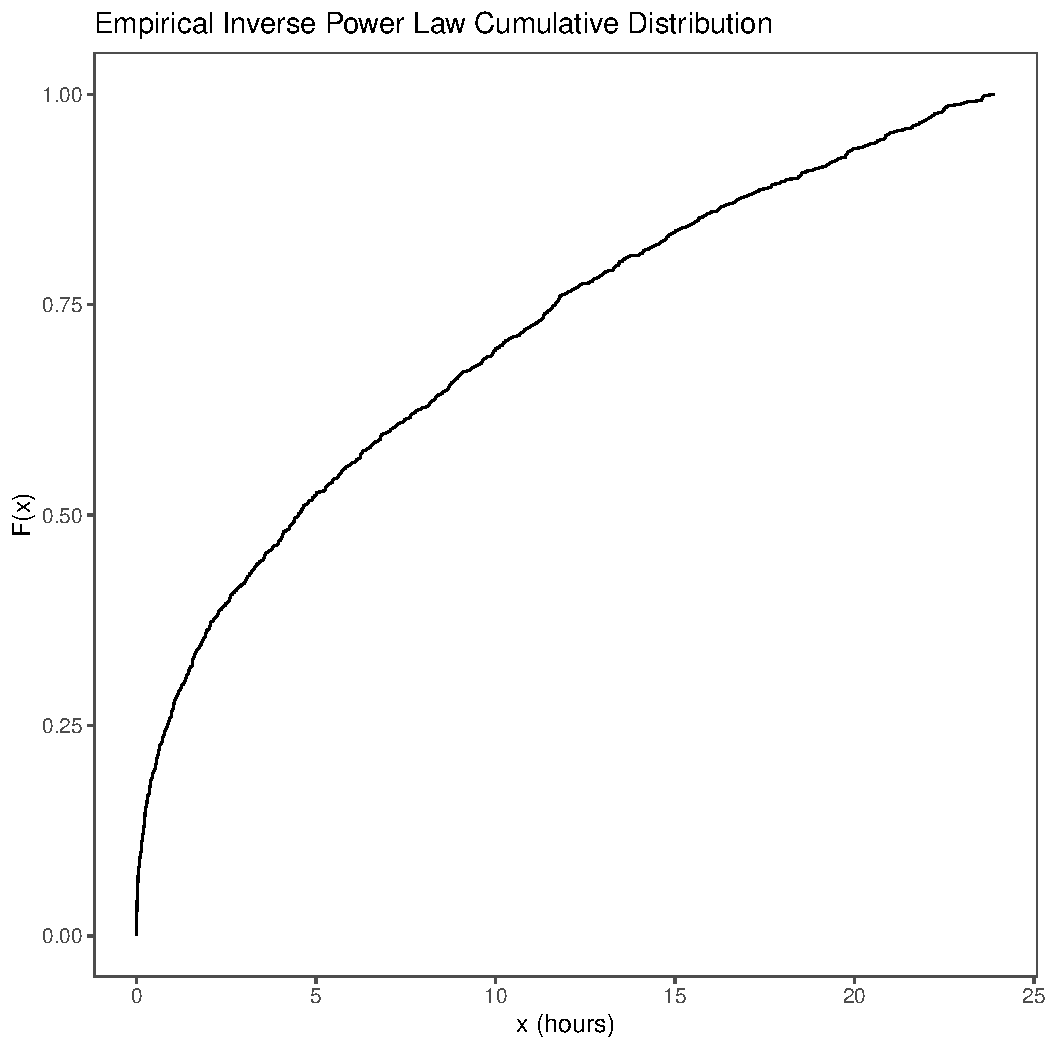
\includegraphics[scale=\patternscale]{figures/comments_power_law}
  \caption{The power-law used to generate comments.}
  \label{figure:comments_dist}
\end{figure}

\begin{figure}[H]
  \centering
  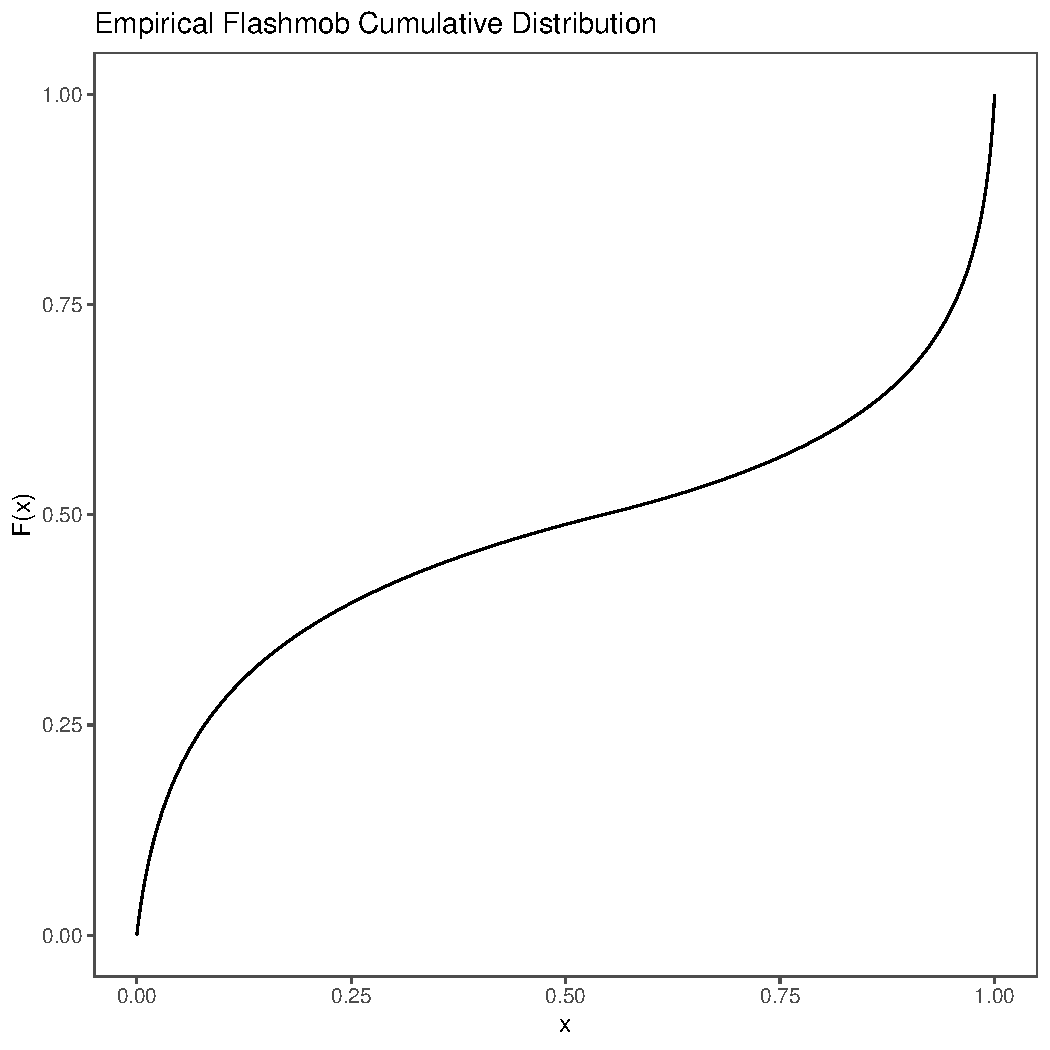
\includegraphics[scale=\patternscale]{figures/flashmob_dist}
  \caption{The distribution used to generate posts during flashmob events.}
  \label{figure:flashmob_dist}
\end{figure}

\subsubsection{Implementation Details}

\datagen is implemented using the MapReduce parallel paradigm. In MapReduce, a
Map function runs on different parts of the input data, in parallel and on many
node clusters. This function processes the input data and produces for each
result a key. Reduce functions then obtain this data and Reducers run in
parallel on many cluster nodes. The produced key simply determines the Reducer
to which the results are sent. The use of the MapReduce paradigm allows the
generator to scale considerably, allowing the generation of huge datasets by
using clusters of machines.

In the case of \datagen, the overall process is divided into three MapReduce jobs.
In the first job, each mapper generates a subset of the persons of the graph. A
key is assigned to each person using one of the similarity functions described
above. Then, reducers receive the key-value pairs sorted by the key,
generate the knows relations following the described windowing process, and
assign to each person a new key based on another similarity function, for the
next MapReduce pass.  This process can be successively repeated for additional
correlation dimension.  Finally, the last reducer generates the remaining
information such as forums, posts and comments.

\subsection{Output Data}

For each scale factor, \datagen produces three different artefacts:
\begin{itemize}
  \item \textbf{Dataset}: The dataset to be bulk loaded by the SUT. It
    corresponds to roughly the 90\% of the total generated network.
  \item \textbf{Update Streams}: A set of update streams containing update
    queries, which are used by the driver to generate the update queries of the
    workloads. This update
    streams correspond to the remaining 10\% of the generated dataset.
  \item \textbf{Substitution Parameters}: A set of files containing the
    different parameter bindings that will be used by the driver to generate the
    read queries of the workloads.
\end{itemize}

\subsubsection{Scale Factors}

\ldbcsnb defines a set of scale factors (SFs), targeting systems of different sizes and budgets.
SFs are computed based on the ASCII size in Gigabytes of the generated output files using the CsvBasic serializer.
For example, SF 1 takes roughly 1~GB in CSV format, SF 3 weights roughly 3~GB and so on and so forth.
The proposed SFs are the following: 1, 3, 10, 30, 100, 300, 1000.
Additionally, two small SFs, 0.1 and 0.3 are provided to help initial validation efforts.

The Test Sponsor may select the SF that better fits their needs, by properly configuring the \datagen, as described in \autoref{section:data_generation}.
The size of the resulting dataset is mainly affected by the following configuration parameters: the number of persons and the number of years simulated.
By default, all SFs are defined over a period of three years, starting from 2010, and SFs are computed by scaling the number of Persons in the network.
\autoref{tab:snsize} shows some metrics of SFs 0.1 \ldots 1000.

\begin{table}[H]
    \small
    \setlength{\tabcolsep}{.5em}
    \centering
    \begin{tabular}{|l||r|r|r|r|r|r|r|r|r|r|r|}
        \hline
        Scale Factor     &     0.1 &     0.3 &        1 &        3 &        10 &        30 &        100 &        300 & \numprint{1000} & \numprint{3000} & \numprint{10000} \\ \hline\hline
        \# Persons       &    1.5K &    3.5K &      11K &      27K &       73K &      182K &       499K &      1.25M &        3.6M & TBD & TBD \\ \hline\hline
        %Number of nodes &  327588 &  908224 &  3181724 &  9281922 &  29987835 &  88789833 &  282637871 &  817316105 &  2686781095 & & \\ \hline
        %Number of edges & 1477965 & 4583118 & 17256038 & 52695735 & 176623445 & 540915404 & 1775513811 & 5269286554 & 17788734714 & & \\ \hline
        \# of nodes      &  327.6K &    908K &     3.2M &     9.3M &       30M &     88.8M &     282.6M &     817.3M &        2.7B & & \\ \hline
        \# of edges      &    1.5M &    4.6M &    17.3M &    52.7M &    176.6M &    540.9M &       1.8B &       5.3B &         17B & & \\ \hline
    \end{tabular}
    \centering
    \caption{Parameters of each scale factor.}
    \label{tab:snsize}
\end{table}

%In \autoref{appendix:scale_factors}, we show the statistics of each of the
%proposed SFs in detail, including distributions for some of the relations.

\begin{table}[htb]
    \scriptsize
    \centering
    \begin{tabular}{|c|p{4.6cm}|p{9.8cm}|}
    	\hline
    	\tableHeaderFirst{C}    & \tableHeader{File}                      & \tableHeader{Content}                                                                   \\
    	\hline\hline
        N                       & organisation\_*.csv                     & id | type({"university", "company"}) | name | url                                       \\
        E                       & organisation\_isLocatedIn\_place\_*.csv & Organisation.id | Place.id                                                              \\
        \hline
        N                       & place\_*.csv                            & id | name | url | type({"city", "country", "continent"})                                \\
        E                       & place\_isPartOf\_place\_*.csv           & Place.id | Place.id                                                                     \\
        \hline
        N                       & tag\_*.csv                              & id | name | url                                                                         \\
        E                       & tag\_hasType\_tagclass\_*.csv           & Tag.id | TagClass.id                                                                    \\
        \hline
        N                       & tagclass\_*.csv                         & id | name | url                                                                         \\
        E                       & tagclass\_isSubclassOf\_tagclass\_*.csv & TagClass.id | TagClass.id                                                               \\
        \hline\hline
        N                       & comment\_*.csv                          & id | creationDate | locationIP | browserUsed | content | length                         \\
        E                       & comment\_hasCreator\_person\_*.csv      & Comment.id | Person.id                                                                  \\
        E                       & comment\_hasTag\_tag\_*.csv             & Comment.id | Tag.id                                                                     \\
        E                       & comment\_isLocatedIn\_place\_*.csv      & Comment.id | Place.id                                                                   \\
        E                       & comment\_replyOf\_comment\_*.csv        & Comment.id | Comment.id                                                                 \\
        E                       & comment\_replyOf\_post\_*.csv           & Comment.id | Post.id                                                                    \\
        \hline
        N                       & forum\_*.csv                            & id | title | creationDate                                                               \\
        E                       & forum\_containerOf\_post\_*.csv         & Forum.id | Post.id                                                                      \\
        E                       & forum\_hasMember\_person\_*.csv         & Forum.id | Person.id | creationDate                                                     \\
        E                       & forum\_hasModerator\_person\_*.csv      & Forum.id | Person.id                                                                    \\
        E                       & forum\_hasTag\_tag\_*.csv               & Forum.id | Tag.id                                                                       \\
        \hline
        N                       & person\_*.csv                           & id | firstName | lastName | gender | birthday | creationDate | locationIP | browserUsed \\
        A                       & person\_email\_emailaddress\_*.csv      & Person.id | email                                                                       \\
        E                       & person\_hasInterest\_tag\_*.csv         & Person.id | Tag.id                                                                      \\
        E                       & person\_isLocatedIn\_place\_*.csv       & Person.id | Place.id                                                                    \\
        E                       & person\_knows\_person\_*.csv            & Person.id | Person.id | creationDate                                                    \\
        E                       & person\_likes\_comment\_*.csv           & Person.id | Post.id | creationDate                                                      \\
        E                       & person\_likes\_post\_*.csv              & Person.id | Post.id | creationDate                                                      \\
        A                       & person\_speaks\_language\_*.csv         & Person.id | language                                                                    \\
        E                       & person\_studyAt\_organisation\_*.csv    & Person.id | Organisation.id | classYear                                                 \\
        E                       & person\_workAt\_organisation\_*.csv     & Person.id | Organisation.id | workFrom                                                  \\
        \hline
        N                       & post\_*.csv                             & id | imageFile | creationDate | locationIP | browserUsed | language | content | length  \\
        E                       & post\_hasCreator\_person\_*.csv         & Post.id | Person.id                                                                     \\
        E                       & post\_hasTag\_tag\_*.csv                & Post.id | Tag.id                                                                        \\
        E                       & post\_isLocatedIn\_place.csv            & Post.id | Place.id                                                                      \\
        \hline
    \end{tabular}
    \caption{Files output by the CsvBasic serializer (33 in total). The first part of the table contains the static entites, the second part contains the dynamic ones. Notation -- C: entity category, N: Node, E: Edge, A: Attribute.}
    \label{table:csv_basic}
\end{table}


\begin{table}[htb]
    \scriptsize
    \centering
    \begin{tabularx}{\linewidth}{|>{\sffamily}c|>{\tt}l|>{\tt}X|}
        \hline
        \tableHeaderFirst{C} & \tableHeader{File}                   & \tableHeader{Content}                                                                                               \\
        \hline\hline
        N                    & organisation\_*.csv                  & id | type | name | url | place                                                                                      \\        \hline
        N                    & place\_*.csv                         & id | name | url | type | isPartOf                                                                                   \\\hline
        N                    & tag\_*.csv                           & id | name | url | hasType                                                                                           \\\hline
        N                    & tagclass\_*.csv                      & id | name | url | isSubclassOf                                                                                      \\\hline\hline
        N                    & comment\_*.csv                       & id | creationDate | locationIP | browserUsed | content | length | creator | place | replyOfPost | replyOfComment    \\
        E                    & comment\_hasTag\_tag\_*.csv          & Comment.id | Tag.id                                                                                                 \\\hline
        N                    & forum\_*.csv                         & id | title | creationDate | moderator                                                                               \\
        E                    & forum\_hasMember\_person\_*.csv      & Forum.id | Person.id | joinDate/creationDate                                                                        \\
        E                    & forum\_hasTag\_tag\_*.csv            & Forum.id | Tag.id                                                                                                   \\\hline
        N                    & person\_*.csv                        & id | firstName | lastName | gender | birthday | creationDate | locationIP | browserUsed | place                     \\
        A                    & person\_email\_emailaddress\_*.csv   & Person.id | email                                                                                                   \\
        E                    & person\_hasInterest\_tag\_*.csv      & Person.id | Tag.id                                                                                                  \\
        E                    & person\_knows\_person\_*.csv         & Person.id | Person.id | creationDate                                                                                \\
        E                    & person\_likes\_comment\_*.csv        & Person.id | Post.id | creationDate                                                                                  \\
        E                    & person\_likes\_post\_*.csv           & Person.id | Post.id | creationDate                                                                                  \\
        A                    & person\_speaks\_language\_*.csv      & Person.id | language                                                                                                \\
        E                    & person\_studyAt\_organisation\_*.csv & Person.id | Organisation.id | classYear                                                                             \\
        E                    & person\_workAt\_organisation\_*.csv  & Person.id | Organisation.id | workFrom                                                                              \\\hline
        N                    & post\_*.csv                          & id | imageFile | creationDate | locationIP | browserUsed | language | content | length | creator | Forum.id | place \\
        E                    & post\_hasTag\_tag\_*.csv             & Post.id | Tag.id                                                                                                    \\\hline
    \end{tabularx}
    \caption{Files output by the CsvMergeForeign serializer (20 in total). The first part of the table contains the static entites, the second part contains the dynamic ones.
        Notation -- \textsf{C}: entity category, \textsf{N}: node, \textsf{E}: edge.}
    \label{table:csv_merge_foreign}
\end{table}


\begin{table}[htb]
    \scriptsize
    \centering
    \begin{tabularx}{\linewidth}{|>{\sffamily}c|>{\tt}l|>{\tt}X|}
        \hline
        \tableHeaderFirst{C} & \tableHeader{File}                      & \tableHeader{Content}                                                                                      \\
        \hline\hline
        N                    & organisation\_*.csv                     & id | type | name | url                                                                                     \\
        E                    & organisation\_isLocatedIn\_place\_*.csv & Organisation.id | Place.id                                                                                 \\
        \hline
        N                    & place\_*.csv                            & id | name | url | type                                                                                     \\
        E                    & place\_isPartOf\_place\_*.csv           & Place.id | Place.id                                                                                        \\
        \hline
        N                    & tag\_*.csv                              & id | name | url                                                                                            \\
        E                    & tag\_hasType\_tagclass\_*.csv           & Tag.id | TagClass.id                                                                                       \\
        \hline
        N                    & tagclass\_*.csv                         & id | name | url                                                                                            \\
        E                    & tagclass\_isSubclassOf\_tagclass\_*.csv & TagClass.id | TagClass.id                                                                                  \\
        \hline\hline
        N                    & comment\_*.csv                          & id | creationDate | locationIP | browserUsed | content | length                                            \\
        E                    & comment\_hasCreator\_person\_*.csv      & Comment.id | Person.id                                                                                     \\
        E                    & comment\_hasTag\_tag\_*.csv             & Comment.id | Tag.id                                                                                        \\
        E                    & comment\_isLocatedIn\_place\_*.csv      & Comment.id | Place.id                                                                                      \\
        E                    & comment\_replyOf\_comment\_*.csv        & Comment.id | Comment.id                                                                                    \\
        E                    & comment\_replyOf\_post\_*.csv           & Comment.id | Post.id                                                                                       \\
        \hline
        N                    & forum\_*.csv                            & id | title | creationDate                                                                                  \\
        E                    & forum\_containerOf\_post\_*.csv         & Forum.id | Post.id                                                                                         \\
        E                    & forum\_hasMember\_person\_*.csv         & Forum.id | Person.id | joinDate                                                               \\
        E                    & forum\_hasModerator\_person\_*.csv      & Forum.id | Person.id                                                                                       \\
        E                    & forum\_hasTag\_tag\_*.csv               & Forum.id | Tag.id                                                                                          \\
        \hline
        N                    & person\_*.csv                           & id | firstName | lastName | gender | birthday | creationDate | locationIP | browserUsed | language | email \\
        E                    & person\_hasInterest\_tag\_*.csv         & Person.id | Tag.id                                                                                         \\
        E                    & person\_isLocatedIn\_place\_*.csv       & Person.id | Place.id                                                                                       \\
        E                    & person\_knows\_person\_*.csv            & Person.id | Person.id | creationDate                                                                       \\
        E                    & person\_likes\_comment\_*.csv           & Person.id | Post.id | creationDate                                                                         \\
        E                    & person\_likes\_post\_*.csv              & Person.id | Post.id | creationDate                                                                         \\
        E                    & person\_studyAt\_organisation\_*.csv    & Person.id | Organisation.id | classYear                                                                    \\
        E                    & person\_workAt\_organisation\_*.csv     & Person.id | Organisation.id | workFrom                                                                     \\
        \hline
        N                    & post\_*.csv                             & id | imageFile | creationDate | locationIP | browserUsed | language | content | length                     \\
        E                    & post\_hasCreator\_person\_*.csv         & Post.id | Person.id                                                                                        \\
        E                    & post\_hasTag\_tag\_*.csv                & Post.id | Tag.id                                                                                           \\
        E                    & post\_isLocatedIn\_place.csv            & Post.id | Place.id                                                                                         \\
        \hline
    \end{tabularx}
    \caption{Files output by the CsvComposite serializer (31 in total). The first part of the table contains the static entites, the second part contains the dynamic ones.
        Notation -- \textsf{C}: entity category, \textsf{N}: node, \textsf{E}: edge.}
    \label{table:csv_composite}
\end{table}


\begin{table}[htb]
    \scriptsize
    \centerline{\begin{tabular}{|c|l|l|}
            \hline
            \tableHeaderFirst{C} & \tableHeader{File}                   & \tableHeader{Content}                                                                                               \\
            \hline\hline
            N                    & organisation\_*.csv                  & id | type | name | url | place                                                                                      \\
            \hline
            N                    & place\_*.csv                         & id | name | url | type| isPartOf                                                                                    \\
            \hline
            N                    & tag\_*.csv                           & id | name | url | hasType                                                                                           \\
            \hline
            N                    & tagclass\_*.csv                      & id | name | url | isSubclassOf                                                                                      \\
            \hline\hline
            N                    & comment\_*.csv                       & id | creationDate | locationIP | browserUsed | content | length | creator | place | replyOfPost | replyOfComment    \\
            E                    & comment\_hasTag\_tag\_*.csv          & Comment.id | Tag.id                                                                                                 \\
            \hline
            N                    & forum\_*.csv                         & id | title | creationDate | moderator                                                                               \\
            E                    & forum\_hasMember\_person\_*.csv      & Forum.id | Person.id | joinDate/creationDate                                                                        \\
            E                    & forum\_hasTag\_tag\_*.csv            & Forum.id | Tag.id                                                                                                   \\
            \hline
            N                    & person\_*.csv                        & id | firstName | lastName | gender | birthday | creationDate | locationIP | browserUsed | place | language | email  \\
            E                    & person\_hasInterest\_tag\_*.csv      & Person.id | Tag.id                                                                                                  \\
            E                    & person\_knows\_person\_*.csv         & Person.id | Person.id | creationDate                                                                                \\
            E                    & person\_likes\_comment\_*.csv        & Person.id | Post.id | creationDate                                                                                  \\
            E                    & person\_likes\_post\_*.csv           & Person.id | Post.id | creationDate                                                                                  \\
            E                    & person\_studyAt\_organisation\_*.csv & Person.id | Organisation.id | classYear                                                                             \\
            E                    & person\_workAt\_organisation\_*.csv  & Person.id | Organisation.id | workFrom                                                                              \\
            \hline
            N                    & post\_*.csv                          & id | imageFile | creationDate | locationIP | browserUsed | language | content | length | creator | Forum.id | place \\
            E                    & post\_hasTag\_tag\_*.csv             & Post.id | Tag.id                                                                                                    \\
            \hline
        \end{tabular}}
    \caption{Files output by the CsvCompositeMergeForeign serializer (18 in total). The first part of the table contains the static entites, the second part contains the dynamic ones. Notation -- C: entity category, N: node, E: edge.}
    \label{table:csv_composite_merge_foreign}
\end{table}


\subsubsection{Dataset}

The datasets are generated in the \texttt{social\_network/} directory, split into static and dynamic parts (\autoref{figure:schema}).
The SUT has to take care only of the generated Dataset to be bulk loaded. Using \texttt{NULL} values for storing optional values is allowed.

The formats currently supported by \datagen serializers are the following:

\begin{itemize}
  \item \textbf{CSV variants:}
      These serializers produce CSV-like text files which use the pipe character ``\texttt{|}'' as the primary field separator and the semicolon character ``\texttt{;}'' as a separator for multi-valued attributes (where applicable).
      The CSV files are stored in two subdirectories: \texttt{static/} and \texttt{dynamic/}.
      Depending on the number of threads used for generating the dataset, the number of files varies, since there is a file generated per thread. We indicate with ``\texttt{*}'' in the specification.
      Currently, the following CSV variants are supported:
    \begin{itemize}
      \item \textbf{CsvBasic:}
      Each entity, relation and attribute with a cardinality larger than one (including attributes \texttt{Person.email} and \texttt{Person.speaks}), are output in a separate file.
      Generated files are summarized in \autoref{table:csv_basic}.

      \item \textbf{CsvMergeForeign:}
      This serializer is similar to CsvBasic, but relations that have a cardinality of 1-to-N are merged in the entity files as a foreign keys.
      There are 13~such relations in total:
      comment\_hasCreator\_person, comment\_isLocatedIn\_place, comment\_replyOf\_comment, comment\_replyOf\_post (merged to Comment);
      forum\_hasModerator\_person (merged to Forum);
      organisation\_isLocatedIn\_place (merged to Organisation);
      person\_isLocatedIn\_place (merged to Person);
      place\_isPartOf\_place (merged to Place);
      post\_hasCreator\_person, post\_isLocatedIn\_place, forum\_containerOf\_post (merged to Post);
      tag\_hasType\_tagclass (merged to Tag);
      tagclass\_isSubclassOf\_tagclass (merged to TagClass).
      Generated files are summarized in \autoref{table:csv_merge_foreign}.

      \item \textbf{CsvComposite:}
      Similar to the CsvBasic format but each entity, and relations with a cardinality larger than one, are output in a separate file.
      Multi-valued attributes (\texttt{Person.email} and \texttt{Person.speaks}) are stored as composite values.
      Generated files are summarized in \autoref{table:csv_composite}.

      \item \textbf{CsvCompositeMergeForeign:}
      Has the traits of both the CsvComposite and the CsvMergeForeign formats.
      Multi-valued attributes (\texttt{Person.email} and \texttt{Person.speaks}) are stored as composite values.
      Generated files are summarized in \autoref{table:csv_composite_merge_foreign}.
    \end{itemize}
  \item \textbf{Turtle:} Dataset in Turtle format for RDF systems.
\end{itemize}

\paragraph{Turtle}

This serializers uses the standard Turtle format\footnote{Description of
the Turtle RDF format http://www.w3.org/TR/turtle/}. It outputs
two files: \texttt{0\_ldbc\_socialnet\_static\_dbp.ttl} and \texttt{0\_ldbc\_socialnet.ttl}, containing the static and the dynamic part of the graph, respectively.

\subsubsection{Update Streams}

\begin{table}[htb]
    \scriptsize
    \centerline{\begin{tabular}{|c|c|c|c|}
        \hline
        start time ($t_\text{s}$) & dependant time ($t_\textrm{d}$) & operation id & \ldots \\
        \hline
    \end{tabular}}
    \caption{
        Generic schema of update (insert) stream files.
        The start time ($t_\text{s}$) is identical to the creationDate attribute (repeated later in the row).}
    \label{table:update_stream_generic_schema}
\end{table}

\begin{table}[htb]
	\scriptsize
	\centerline{\begin{tabular}{|l|}
		\hline
		$t_\text{s}$ | $t_\textrm{d}$ | 1 | personId | personFirstName | personLastName | gender | birthday | creationDate | locationIP | browserUsed | cityId | languages | emails | tagIds | studyAt | workAt \\\hline
		$t_\text{s}$ | $t_\textrm{d}$ | 2 | personId | postId | creationDate \\\hline
		$t_\text{s}$ | $t_\textrm{d}$ | 3 | personId | commentId | creationDate \\\hline
		$t_\text{s}$ | $t_\textrm{d}$ | 4 | forumId | forumTitle | creationDate | moderatorPersonId | tagIds \\\hline
		$t_\text{s}$ | $t_\textrm{d}$ | 5 | forumId | personId | creationDate \\\hline
		$t_\text{s}$ | $t_\textrm{d}$ | 6 | postId | imageFile | creationDate | locationIP | browserUsed | language | content | length | authorPersonId | forumId | countryId | tagIds \\\hline
		$t_\text{s}$ | $t_\textrm{d}$ | 7 | commentId | creationDate | locationIP | browserUsed | content | length | authorPersonId | countryId | replyToPostId | replyToCommentId | tagIds \\\hline
		$t_\text{s}$ | $t_\textrm{d}$ | 8 | person1Id | person2Id | creationDate \\
		\hline
	\end{tabular}}
	\caption{Schemas of the lines in the update (insert) stream files.}
	\label{table:update_stream_schemas}
\end{table}


The generic schema is given in \autoref{table:update_stream_generic_schema}, while the concrete schema of each insert operation is given in \autoref{table:update_stream_schemas}.
The update stream files are generated in the \texttt{social\_network/} directory and are grouped as follows:

\begin{itemize}
    \item \texttt{updateStream\_*\_person.csv} contains update operation 1: \queryRefCard{interactive-insert-01}{II}{1}
    \item \texttt{updateStream\_*\_forum.csv} contains update operations 2--8: %
    \queryRefCard{interactive-insert-02}{II}{2}
    \queryRefCard{interactive-insert-03}{II}{3}
    \queryRefCard{interactive-insert-04}{II}{4}
    \queryRefCard{interactive-insert-05}{II}{5}
    \queryRefCard{interactive-insert-06}{II}{6}
    \queryRefCard{interactive-insert-07}{II}{7}
    \queryRefCard{interactive-insert-08}{II}{8}
\end{itemize}

Remark: update streams in version 0.3.0 only contain inserts. Delete operations are being designed and will be released later.

\subsubsection{Substitution Parameters}

The substitution parameters are generated in the \texttt{substitution\_parameters/} directory.
Each parameter file is named \texttt{\{interactive|bi\}\_<id>\_param.txt}, corresponding to an operation of
Interactive complex reads (\queryRefCard{interactive-complex-read-01}{IC}{1}--\queryRefCard{interactive-complex-read-14}{IC}{14}) and
BI reads (\queryRefCard{bi-read-01}{BI}{1}--\queryRefCard{bi-read-25}{BI}{25}).
The schemas of these files are defined by the operator, e.g. the schema of \queryRefCard{interactive-complex-read-01}{IC}{1} is ``\texttt{personId|firstName}''.

%%%%%%%%%%%%%%%%%%%%%%%%%%%%%%%%%%%%%%%%%%%%%%%%%%%%%%%%%%%%%%%%%%%%%%%%%%%%%%
%%%%%%%%%%%%%%%%%%%%%%%%%%%%%%%%%%%%%%%%%%%%%%%%%%%%%%%%%%%%%%%%%%%%%%%%%%%%%%
%%%%%%%%%%%%%%%%%%%%%%%%%%%%%%%%%%%%%%%%%%%%%%%%%%%%%%%%%%%%%%%%%%%%%%%%%%%%%%

\section{Benchmark Workflow}
\label{section:workflow}

The workflow of the benchmark is shown in \autoref{figure:workflow}.

\begin{figure}[htb]
    \centering
    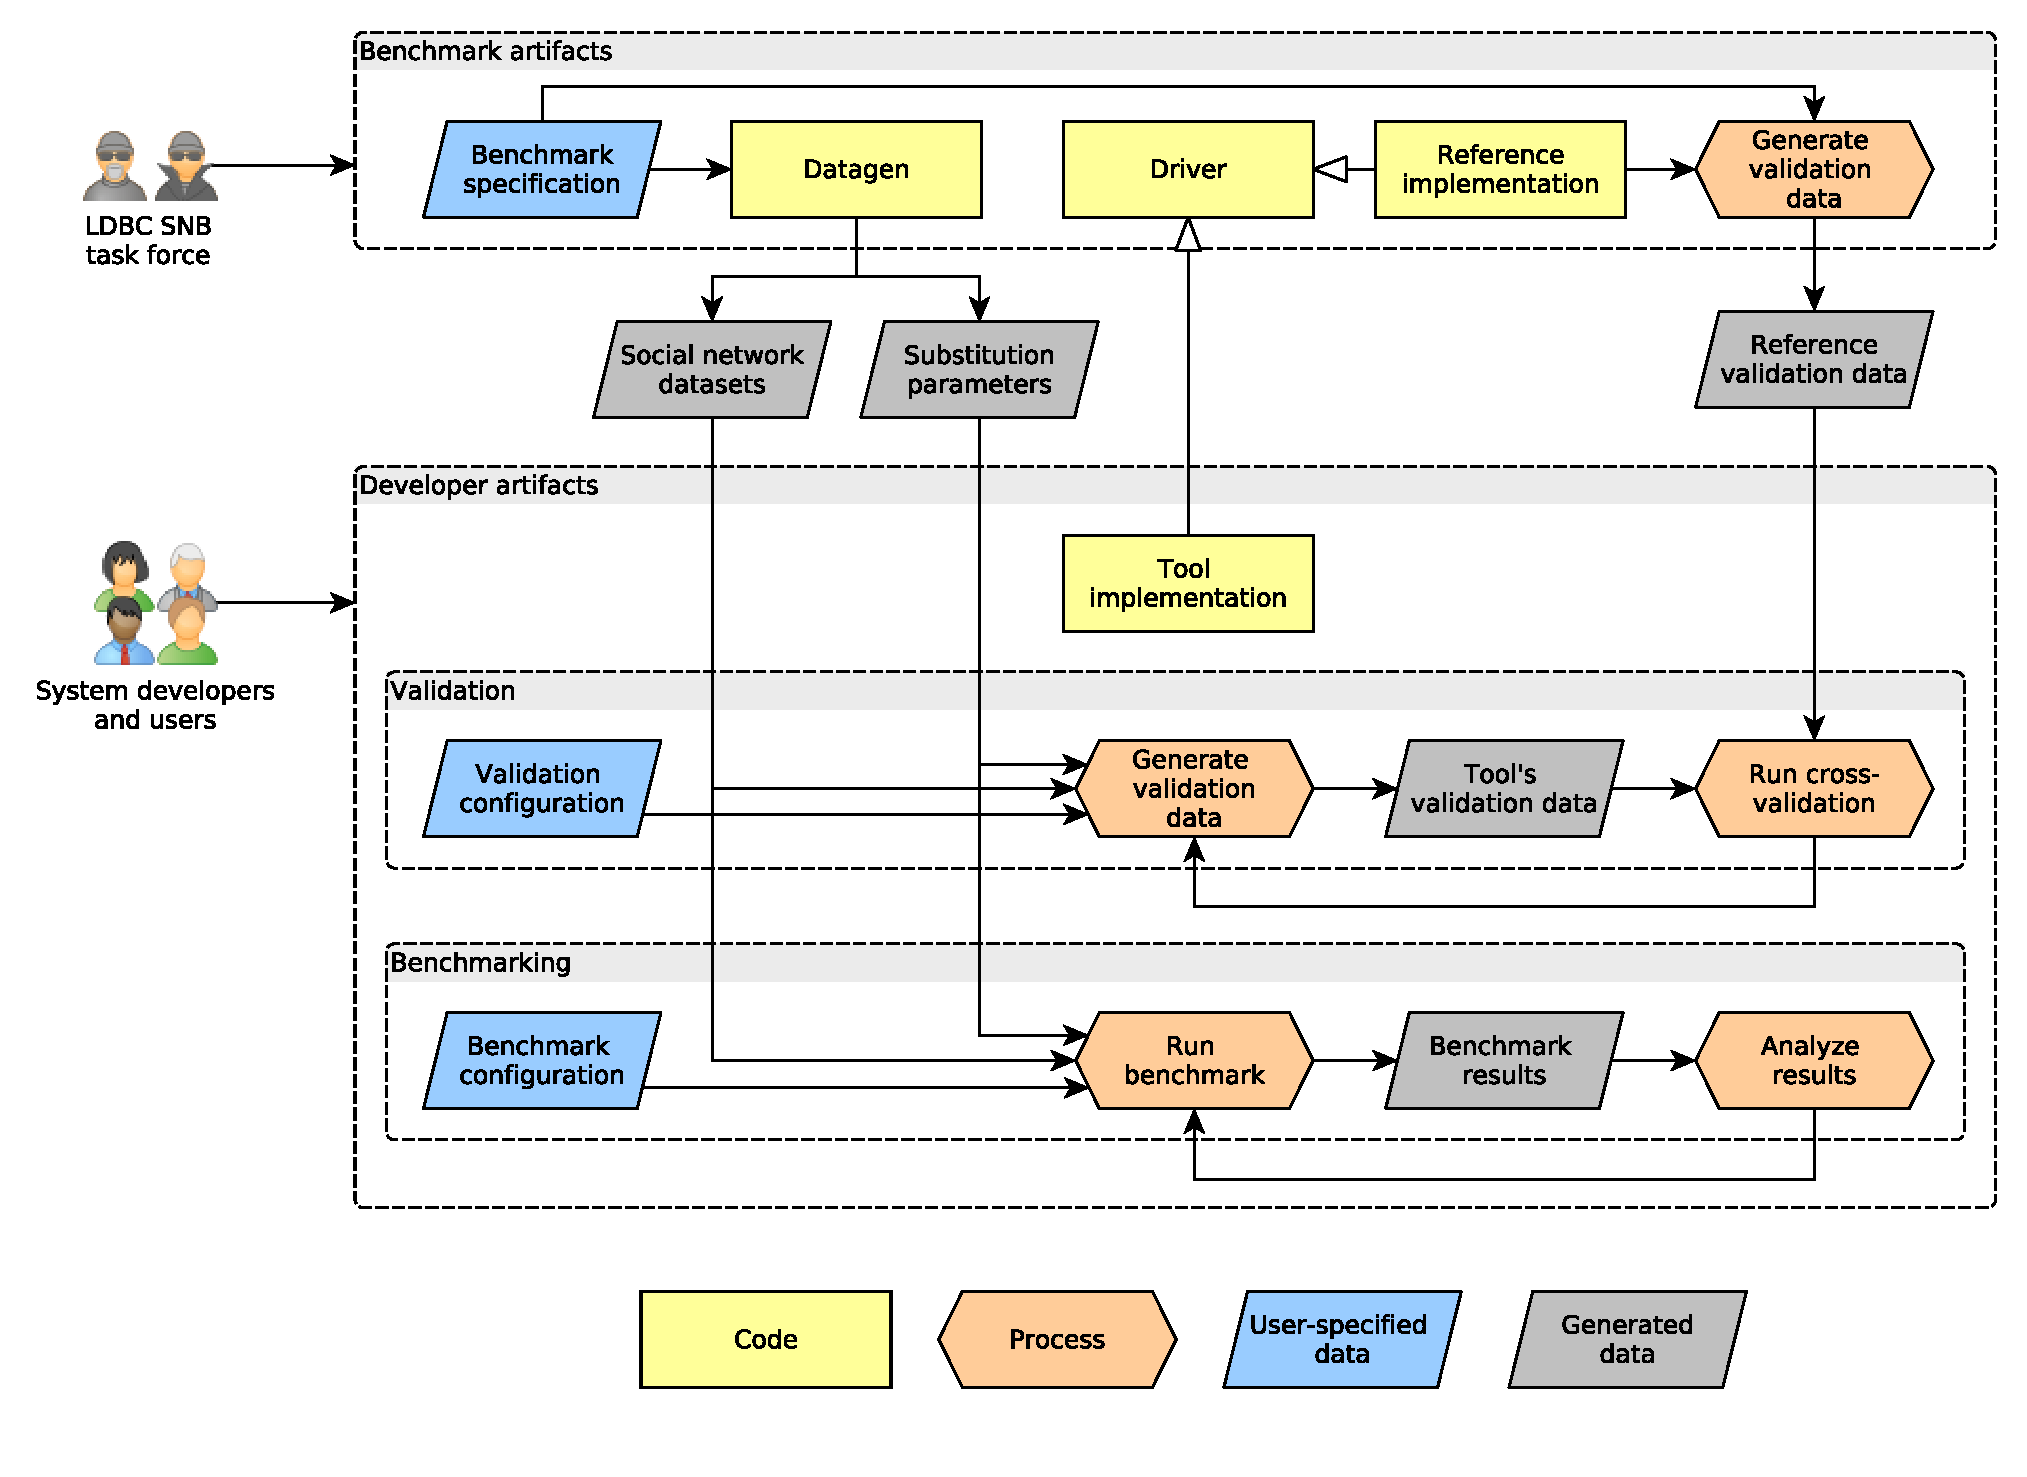
\includegraphics[width=\linewidth]{figures/workflow}
    \caption{Benchmark workflow.}
    \label{figure:workflow}
\end{figure}
